\documentclass[conference]{IEEEtran}
\IEEEoverridecommandlockouts
\usepackage{cite}
\usepackage{amsmath,amssymb,amsfonts}
\usepackage{graphicx}
\usepackage{textcomp}
\usepackage{booktabs}
\usepackage{array}
\usepackage{placeins}
\usepackage{balance}
\usepackage{capt-of}
\usepackage{tabularx}
\usepackage{ragged2e}
\usepackage{microtype}
\hyphenation{Magna-Tag-A-Tune You-Tube Graph-SAGE Tiny-BERT Info-NCE Music-Caps}
\renewcommand{\topfraction}{0.9}
\renewcommand{\bottomfraction}{0.8}
\renewcommand{\textfraction}{0.08}
\renewcommand{\floatpagefraction}{0.75}
\setcounter{topnumber}{4}
\setcounter{totalnumber}{6}
\usepackage[hidelinks]{hyperref}
\graphicspath{{../results/plots/}}

\title{GNN-Based BERT for Understanding Context from Music}

\author{\IEEEauthorblockA{\textit{CSE425 / EEE474 / CSE715 --- Neural Networks}\\
September 2026}}

\begin{document}
\maketitle

\begin{abstract}
Music context is jointly harmonic, timbral, and linguistic. We implement a four-task hybrid of TinyBERT and GraphSAGE: multi-label tagging from captions, message passing on segment-similarity and chord-transition graphs, cross-attention fusion with valence/arousal heads, and dual-encoder InfoNCE retrieval. Experiments use a genre-balanced subset of FMA-small: 511 clips of 30\,s, 386 artists, and artist-disjoint splits $327/94/90$. Captions come from FMA metadata. MusicCaps audio and DEAM ratings are not available, so tags are keyword-mapped from those captions and emotion targets follow genre priors. On 90 held-out tracks, concat fusion reaches macro-F1 $0.783$ versus $0.772$ (BERT), $0.264$ (GNN), and $0.255$ (CNN). Caption-to-audio R@5 is $0.078$ against chance $0.056$. The main result is the gap between metadata-derived text tags and real FMA audio, not a claim of MusicCaps-level caption understanding.
\end{abstract}

\begin{IEEEkeywords}
graph neural networks, BERT, music tagging, contrastive learning, Free Music Archive
\end{IEEEkeywords}

\section{Introduction}
A recording can be folk, acoustic, guitar-led, and built from a short chord loop at the same time. Convolutional taggers on log-mel spectrograms capture local timbre but not chord transitions or repeated segments. Language models on captions capture semantics but not when those words align with a modulation or a drop. The course assignment therefore asks for a hybrid: a BERT encoder on text, a graph neural network on a structure graph extracted from audio, a fusion stage that produces a context vector, and an optional contrastive retriever.

We represent each track as a tuple of spectrogram, caption, graph, and labels. Task~1 contextualizes the caption with a Transformer encoder and predicts 24 MagnaTagATune-style tags. Task~2 message-passes on two graphs built from the same clip: a segment-similarity graph over 1\,s windows and a chord-transition graph over estimated major/minor triads. Task~3 fuses the graph readout with token states for tags and continuous valence/arousal. Task~4 aligns graph and caption towers with InfoNCE. The objective is understanding, not generation.

This paper reports an end-to-end run on official FMA-small audio rather than a synthetic stand-in. Our contributions are: (i)~loaders, SHA1-checked download, and a 511-clip genre-balanced subset with artist-disjoint splits; (ii)~dense batched GraphSAGE/GAT, TinyBERT, concat and cross-attention fusion, and a dual encoder, all without PyTorch Geometric; (iii)~majority, random, CNN, BERT-only, and GNN-only baselines with held-out metrics; (iv)~saved \texttt{.pt} graphs and a demo notebook. All tables below are from that FMA run.

\section{Related Work}
BERT~\cite{devlin2019} contextualizes tokens with bidirectional self-attention. We keep the \texttt{[CLS]} interface so a HuggingFace checkpoint can replace our two-layer encoder, but we train TinyBERT from scratch: 511 clips do not support masked-language pretraining of a full BERT. GraphSAGE~\cite{hamilton2017} samples and aggregates neighbourhoods; GAT~\cite{velickovic2018} replaces the mean with learned attention. Both appear in the assignment. We implement them as dense batched layers over padded adjacency, which is enough for graphs of 30 nodes.

FMA~\cite{defferrard2017} supplies Creative Commons audio, artist identifiers, and a top-genre field. MagnaTagATune~\cite{law2009} is a crowd-tagged clip collection; we use a 24-tag subset of its typical inventory (instruments, mood, production, key, tempo) because the full MTT dump is not on disk. MusicCaps~\cite{agostinelli2023} pairs YouTube excerpts with expert captions; we store the public CSV but do not download YouTube audio. DEAM~\cite{aljanaki2017} provides human valence/arousal; it is gated, so emotion targets in this paper are genre priors. InfoNCE~\cite{oord2018} is the standard contrastive retrieval loss. Spectrogram CNNs remain a strong MIR baseline; our three-block mel CNN is that control.

Graph representations of music usually encode either beats, chroma, or functional harmony. Our segment graph is closer to a self-similarity matrix with a temporal backbone. The chord graph is a first-order Markov chain on 24 triad templates. Neither claims to be a musicological parse; both are deterministic functions of the spectrogram so that Task~2 has a well-defined $G$.

\section{Problem Formulation}
$X_{\mathrm{audio}}$ is a 128-bin log-mel spectrogram at $22\,050$\,Hz (hop 512), plus 12-bin chroma, 13 MFCCs, RMS, spectral centroid, and zero-crossing rate. Each feature is $z$-scored per clip. $X_{\mathrm{text}}$ is a whitespace-tokenized caption of at most 48 tokens with \texttt{[CLS]}/\texttt{[SEP]} and padding. $G=(V,E)$ is either a \emph{segment graph} or a \emph{chord-transition graph}, defined in Section~\ref{sec:graphs}. Labels $y$ comprise 24 binary tags, an 8-way genre, and valence/arousal in $[0,1]$.

BERT maps tokens to $H_{\mathrm{text}}\in\mathbb{R}^{L\times d}$ and a CLS vector $t$. GraphSAGE updates
\begin{equation}
h_i^{(l+1)}=\sigma\Big(W^{(l)}\cdot\mathrm{CONCAT}\big(h_i^{(l)},\mathrm{MEAN}_{j\in N(i)}h_j^{(l)}\big)\Big).
\end{equation}
In the dense implementation the adjacency $A$ is already symmetrically normalized with self-loops, so $Ah$ is a mean-like aggregate and the layer is $\mathrm{ReLU}(W[h;Ah])$. A node mask zeros padded rows before mean pooling to a graph vector $g$. Fusion produces $z=\mathrm{Fusion}(g,H_{\mathrm{text}})$ and $\hat{y}=\sigma(Wz+b)$. Tagging uses binary cross-entropy. Task~3 adds $\alpha\|v-\hat{v}\|_2^2+\beta\|a-\hat{a}\|_2^2$ with $\alpha=\beta=0.35$.

The eight assignment genres are jazz, rock, classical, electronic, hip-hop, pop, metal, and folk. FMA-small's top genres do not include jazz or metal; those two heads are unused in this run (Section~\ref{sec:data}). The 24 tags are guitar, piano, drums, synth, vocals, strings, bass, brass, melancholic, energetic, calm, dark, uplifting, danceable, instrumental, acoustic, electronic\_prod, live, 1960s, modern, major\_key, minor\_key, fast\_tempo, and slow\_tempo.

\section{Method}

\subsection{Task 1: BERT Tag Classifier}
A two-layer pre-norm Transformer (hidden 64, four heads, GELU, dropout $0.15$) implements the assignment's Algorithm~1. Token embedding, learned positional embedding, and a padding mask are standard. The classification head is dropout-linear from the CLS state to 24 logits, trained with BCE. \texttt{TinyMusicBERT} returns both the full $H_{\mathrm{text}}$ and $t_{\mathrm{cls}}$, matching HuggingFace BERT's last hidden state and pooled output. Setting \texttt{model.hf\_name} in \texttt{config.yaml} swaps the backbone without touching fusion or contrastive code. The vocabulary is rebuilt from the current captions before training so FMA titles and artist names are in-vocab.

\subsection{Task 2: Graphs and GraphSAGE}
\label{sec:graphs}
Dense batched GraphSAGE (two layers, hidden 64) and an optional GAT layer operate on padded graphs. We train an 8-way genre head (cross-entropy) and a 24-tag head (BCE) from the same encoder weights copied into two classifiers. GAT uses two heads, LeakyReLU $0.2$, and adjacency as an attention mask:
\begin{equation}
\begin{aligned}
e_{ij}&=\mathrm{LeakyReLU}\big(a^{\top}[Wh_i;Wh_j]\big),\\
\alpha_{ij}&=\mathrm{softmax}_{j\in N(i)}(e_{ij}).
\end{aligned}
\end{equation}
The default run uses GraphSAGE. A three-block CNN ($16$--$32$--$64$ channels, $64\times 32$ log-mel) is the spectrogram baseline: no graph, no text.

\paragraph{Segment graph.}
A 30\,s crop yields $N=30$ windows of 1\,s. Node $i$ holds the concatenation of mean and standard deviation of log-mel, chroma, MFCC, RMS, centroid, and ZCR over that window ($312$ dimensions). Adjacent windows receive a temporal edge. If $\cos(u_i,u_j)>\tau=0.62$ on the chroma$\|$MFCC slice, a similarity edge is added. Self-loops are kept. With $A_{ij}=w_{ij}$ the unnormalized weights,
\begin{equation}
\hat{A}=D^{-1/2}(A+I)D^{-1/2},\quad
D_{ii}=\sum_j(A+I)_{ij}.
\end{equation}

\paragraph{Chord graph.}
Frame-wise chroma is $\ell_2$-normalized and matched to 24 templates (12 major and 12 minor triads, cosine). Consecutive identical chord indices collapse to one node. An edge $u\to v$ records how often chord $u$ is followed by $v$; weights are counts. Isolated chords keep a self-loop. Average size on this subset is $8.3$ nodes.

\subsection{Task 3: GNN--BERT Fusion}
Cross-attention treats the graph vector as a single query against caption keys and values:
\begin{equation}
Q=gW_Q,\quad K=H_{\mathrm{text}}W_K,\quad V=H_{\mathrm{text}}W_V,
\end{equation}
\begin{equation}
A=\mathrm{softmax}(QK^{\top}/\sqrt{d}),\qquad
z=\mathrm{MLP}([g;\,AV]).
\end{equation}
Padding tokens are masked with $-10^{9}$ before the softmax. The MLP is dropout--linear--GELU--dropout back to dimension 64. Three linear heads read $z$: 24 tag logits, scalar valence, and scalar arousal (no sigmoid on VA; targets already lie in $[0,1]$). The early-concat ablation replaces the attention pool with $[g;t_{\mathrm{CLS}}]$ and the same MLP. BERT weights are warm-started from Task~1 when the checkpoint exists.

\subsection{Task 4: Contrastive Dual Encoder}
A GraphSAGE tower and a TinyBERT tower each project to a 64-d sphere through a two-layer GELU MLP. Symmetric InfoNCE with temperature $\tau=0.07$ is
\begin{equation}
\mathcal{L}_{\mathrm{NCE}}=-\log\frac{\exp(\mathrm{sim}(g_i,t_i)/\tau)}{\sum_j\exp(\mathrm{sim}(g_i,t_j)/\tau)},
\end{equation}
averaged with the transposed batch. $\mathrm{sim}$ is cosine similarity. Retrieval metrics are R@1, R@5, and R@10 on the 90 held-out pairs, in both caption-to-audio and audio-to-caption directions. Chance R@5 is $5/90\approx 0.056$.

\section{Experimental Setup}
\label{sec:data}

\subsection{Corpus}
FMA metadata and FMA-small are fetched from the official SWITCH mirror~\cite{defferrard2017} and SHA1-checked by the download script. We take a seed-42, genre-balanced subset: 64 clips from each of the eight FMA-small top genres. One mp3 failed to decode, leaving 511 tracks from 386 artists, each resampled to $22\,050$\,Hz and cropped to 30\,s from the start of the file.

FMA-small labels map onto the assignment inventory by sending Experimental to electronic, International to folk, and Instrumental to classical; the other five top genres keep their names. After mapping, the corpus contains 128 folk, 128 electronic, 64 rock, 64 pop, 64 classical, and 63 hip-hop clips (Table~\ref{tab:genre}). Jazz and metal have zero examples.

Captions follow a short template: genre, title, artist, album, and ``Free Music Archive.'' Tags are keyword-mapped from that text, FMA tag strings, leaf genre names, and genre priors (mean $6.24$ positives per clip). The MusicCaps CSV is on disk (5\,521 rows) but has no audio, so it is not joined. DEAM is absent; valence and arousal are mapped genre priors. Splits are artist-disjoint: $327$ train, $94$ val, $90$ test. Table~\ref{tab:data} states what this run actually uses. If FMA audio is missing, a 288-clip synthetic generator still runs the pipeline offline. Tables~\ref{tab:results}--\ref{tab:qual} are \emph{not} from that generator.

\begin{table}[t]
\caption{Mapped genre counts in the 511-clip FMA subset.}
\label{tab:genre}
\centering
\setlength{\tabcolsep}{4pt}
\begin{tabular}{@{}lcc@{}}
\toprule
Mapped genre & Clips & FMA-small source \\
\midrule
folk & 128 & Folk + International \\
electronic & 128 & Electronic + Experimental \\
rock & 64 & Rock \\
pop & 64 & Pop \\
classical & 64 & Instrumental \\
hip-hop & 63 & Hip-Hop (one decode fail) \\
jazz / metal & 0 & not in FMA-small top genres \\
\bottomrule
\end{tabular}
\end{table}

\begin{table}[t]
\caption{Sources used in this paper versus the assignment table. MTT is MagnaTagATune.}
\label{tab:data}
\centering
\renewcommand{\arraystretch}{1.18}
\setlength{\tabcolsep}{3pt}
\begin{tabularx}{\columnwidth}{@{}>{\raggedright\arraybackslash}p{2.15cm}>{\raggedright\arraybackslash}X>{\raggedright\arraybackslash}X@{}}
\toprule
Source & On disk & Role \\
\midrule
FMA-small & 511 mp3s + metadata & audio, genre, splits, captions \\
MusicCaps & CSV only, no audio & unused for training \\
DEAM & absent (gated) & VA from genre priors \\
MTT & absent & 24-tag inventory \\
GTZAN & absent & loader only \\
\bottomrule
\end{tabularx}
\end{table}

\FloatBarrier

\subsection{Training and Metrics}
AdamW, learning rate $1.5\times 10^{-3}$, weight decay $10^{-4}$, batch size 16, dropout $0.15$, CPU, PyTorch 2.14. Epochs: 10 (BERT), 14 (GNN, CNN, fusion), 16 (contrastive). Graphs are padded to the longest graph in the minibatch; a binary mask marks real nodes. The vocabulary is rebuilt from FMA captions before Task~1. Best validation checkpoints (macro-F1 for tags, accuracy for genre, R@5 for retrieval, F1 minus a penalty on emotion MAE for fusion) are restored before test evaluation. Seed 42. Table~\ref{tab:hp} lists the remaining knobs.

Multi-label tagging is scored with macro-F1, micro-F1, and area under the precision--recall curve. Emotion uses mean absolute error averaged over valence and arousal, plus $R^2$. Genre is top-1 accuracy. Retrieval is Recall@$K$ on the 90 aligned test pairs. Random tags draw uniform scores; majority tags copy the train empirical frequency.

\begin{table}[t]
\caption{Architecture and optimization (from \texttt{config.yaml}).}
\label{tab:hp}
\centering
\renewcommand{\arraystretch}{1.12}
\setlength{\tabcolsep}{4pt}
\begin{tabularx}{\columnwidth}{@{}lX@{}}
\toprule
Item & Value \\
\midrule
Sample rate / crop & $22\,050$\,Hz / 30\,s \\
Segment / $\tau$ & 1\,s / $0.62$ \\
Node dim / chord nodes & 312 / $8.3$ mean \\
TinyBERT & 2 layers, $d{=}64$, 4 heads, $L{=}48$ \\
GraphSAGE & 2 layers, $d{=}64$, mean pool \\
CNN & $16,32,64$ on $64\times 32$ mel \\
Optimiser & AdamW $1.5\times 10^{-3}$, wd $10^{-4}$ \\
Batch / dropout & 16 / $0.15$ \\
InfoNCE $\tau$ / emotion & $0.07$ / $\alpha=\beta=0.35$ \\
Device / seed & CPU / 42 \\
\bottomrule
\end{tabularx}
\end{table}

\section{Results}

\begin{table}[t]
\caption{Held-out artist split ($N=90$). Chance caption$\to$audio R@5 is $5/90\approx 0.056$.}
\label{tab:results}
\centering
\scriptsize
\setlength{\tabcolsep}{3.2pt}
\begin{tabular}{@{}lcccc@{}}
\toprule
Model & F1$_{\mathrm{mac}}$ & F1$_{\mathrm{mic}}$ & AUC-PR & MAE \\
\midrule
Random & 0.000 & 0.000 & 0.319 & --- \\
Majority & 0.118 & 0.420 & 0.297 & --- \\
CNN mel & 0.255 & 0.489 & 0.524 & --- \\
BERT-only & 0.772 & 0.950 & 0.858 & --- \\
GNN-only & 0.264 & 0.521 & 0.516 & --- \\
Concat fusion & \textbf{0.783} & \textbf{0.957} & \textbf{0.868} & 0.039 \\
Cross-attn & 0.779 & 0.953 & 0.860 & \textbf{0.037} \\
\bottomrule
\end{tabular}
\end{table}

\begin{table}[t]
\caption{Genre accuracy and retrieval on the same 90 clips.}
\label{tab:aux}
\centering
\scriptsize
\setlength{\tabcolsep}{3pt}
\begin{tabular}{@{}lccc@{}}
\toprule
Model & Genre acc. & C$\to$A @1/5/10 & A$\to$C @1/5/10 \\
\midrule
CNN & \textbf{0.489} & --- & --- \\
GNN & 0.422 & --- & --- \\
InfoNCE & --- & 0.00/\textbf{0.08}/0.12 & 0.01/0.04/0.12 \\
\bottomrule
\end{tabular}
\end{table}

Table~\ref{tab:results} and Table~\ref{tab:aux} summarize the test split. Audio-only models sit near $0.26$ macro-F1: FMA-small is a noisy tagging problem at this capacity. The CNN slightly beats GraphSAGE on 8-way genre ($0.489$ vs.\ $0.422$), which is expected for a 30-node chroma graph versus a spectrogram CNN that sees the full time--frequency plane. BERT is strong because the 24 tags are constructed from the same metadata that forms the caption, so Task~1 is closer to decoding a template than to open-vocabulary MusicCaps tagging. Concat fusion still records the best tag F1 ($0.783$ vs.\ $0.772$ BERT) and is the only model that jointly regresses valence/arousal. Cross-attention is $0.004$ F1 behind concat and $0.002$ MAE better on emotion. Emotion MAE looks small ($0.037$) because the targets are genre priors, which both the caption and the graph can recover; $R^2$ is $0.82$ valence / $0.91$ arousal for cross-attention. This is not a DEAM human-rating result.

Contrastive R@5 is $0.078$ caption-to-audio and $0.044$ audio-to-caption, only slightly above chance. FMA captions are short and stereotyped (``A $g$ recording titled $t$ by $a$ \ldots''), so many queries share nearly the same bag of tokens. Rank-1 is often a same-genre neighbour, not the paired identifier.

Fig.~\ref{fig:f1} shows validation macro-F1 versus epoch: text models jump once the caption template is decoded, while GNN and CNN climb slowly on audio. Fig.~\ref{fig:ablation} makes the same split visible as a test ablation. Fig.~\ref{fig:tsne} shows the fusion vector $z$; structure follows mapped genre and prior-based mood quadrants. Fig.~\ref{fig:va} plots predicted versus true VA, with rings near the genre-prior centres.

\begin{figure}[tb]
\centering
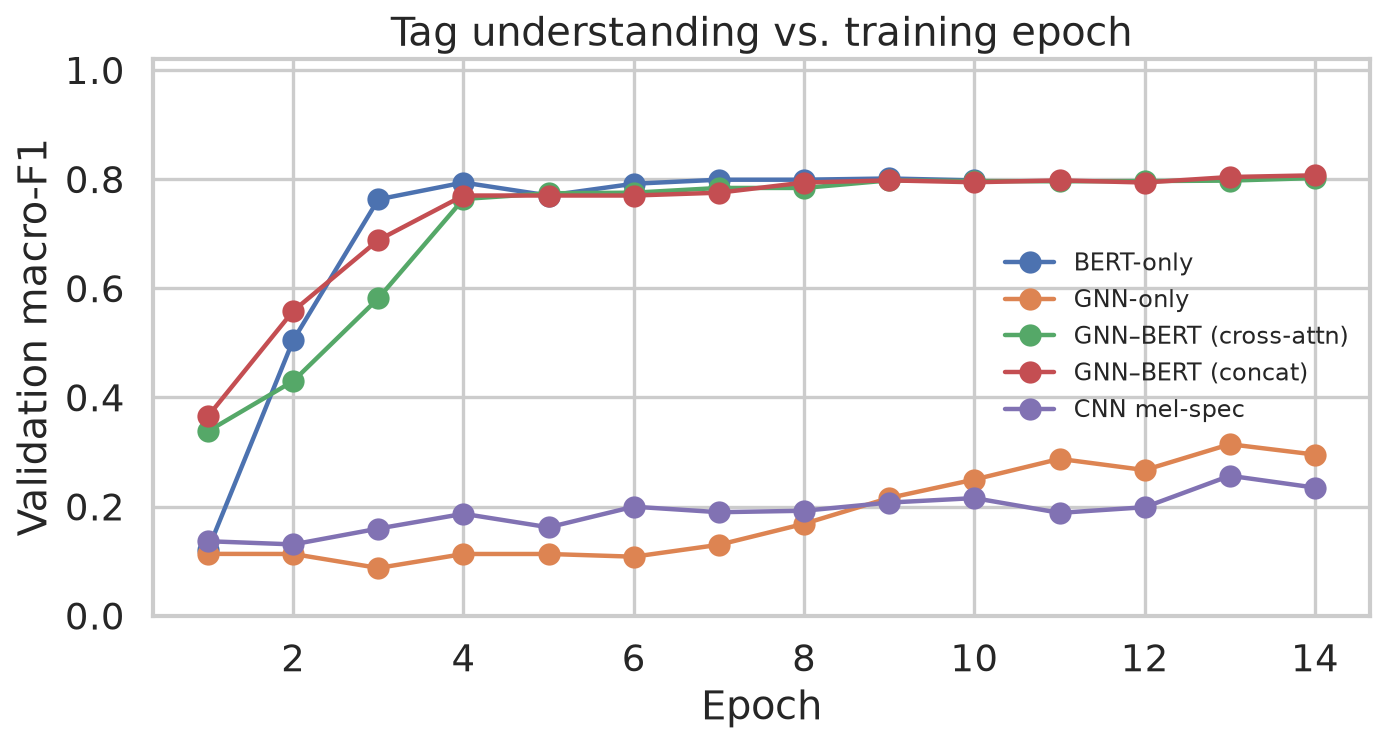
\includegraphics[width=\columnwidth,height=1.42in,keepaspectratio]{f1_curves.png}
\caption{Validation macro-F1 versus epoch. BERT and fusion rise once caption templates are decoded; GNN and CNN improve slowly on audio.}
\label{fig:f1}
\end{figure}

\begin{figure}[tb]
\centering
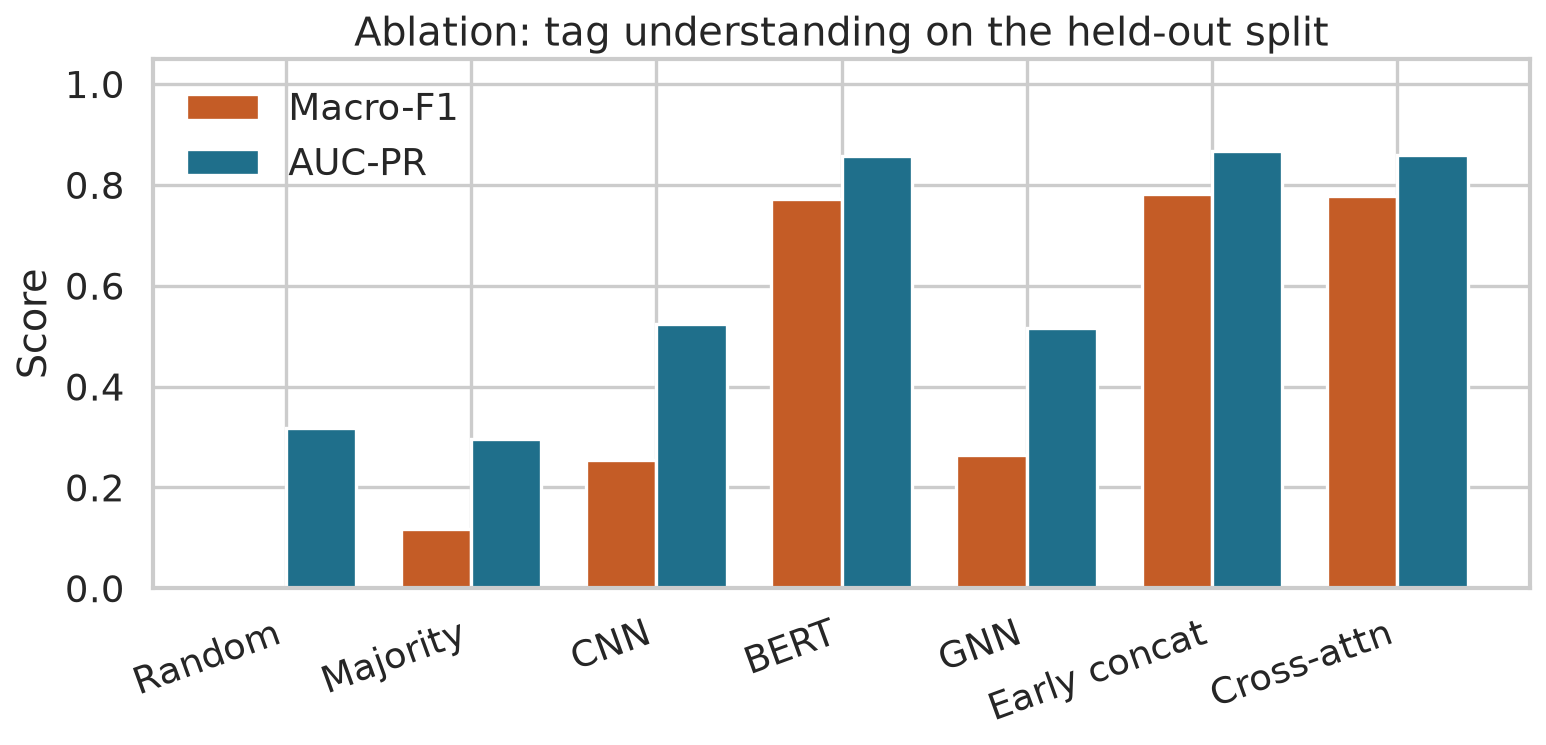
\includegraphics[width=\columnwidth,height=1.42in,keepaspectratio]{ablation.png}
\caption{Test ablation of macro-F1 and AUC-PR. Text towers dominate; audio-only bars are the honest FMA result.}
\label{fig:ablation}
\end{figure}

\begin{figure}[tb]
\centering
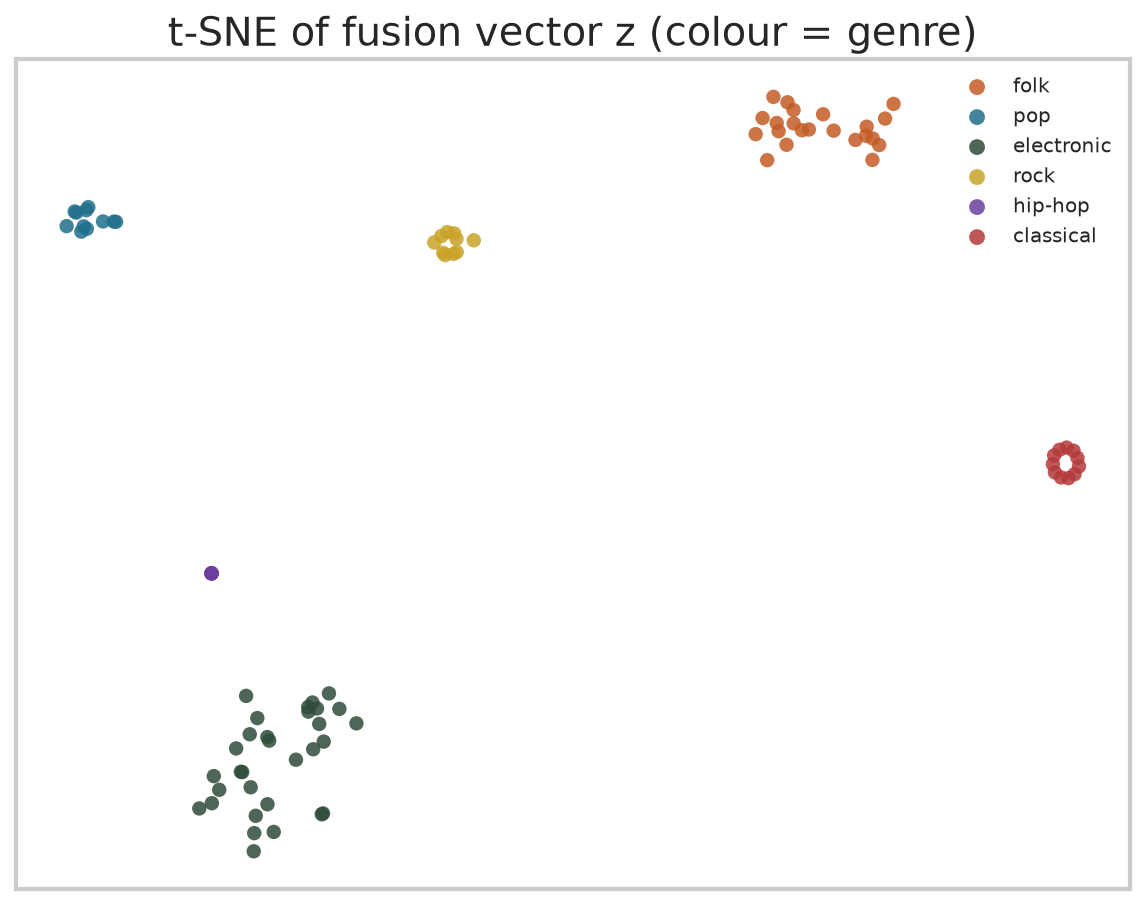
\includegraphics[width=\columnwidth,height=1.42in,keepaspectratio]{tsne_genre.png}\\[-2pt]
{\scriptsize (a) Colour $=$ mapped genre}\\[6pt]
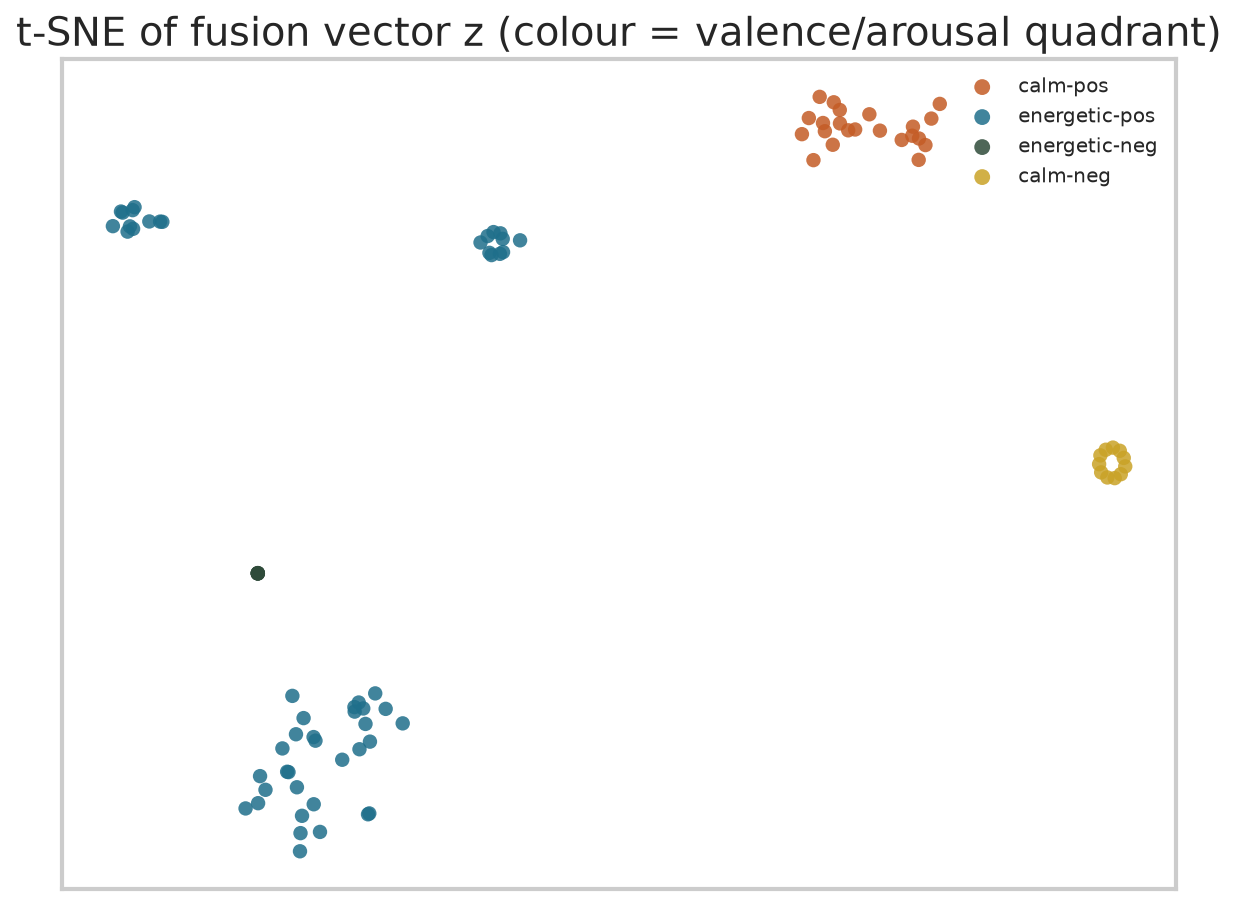
\includegraphics[width=\columnwidth,height=1.42in,keepaspectratio]{tsne_mood.png}\\[-2pt]
{\scriptsize (b) Colour $=$ valence/arousal quadrant (genre-prior VA, not DEAM)}
\caption{t-SNE of the fusion vector $z$.}
\label{fig:tsne}
\end{figure}

\begin{figure}[tb]
\centering
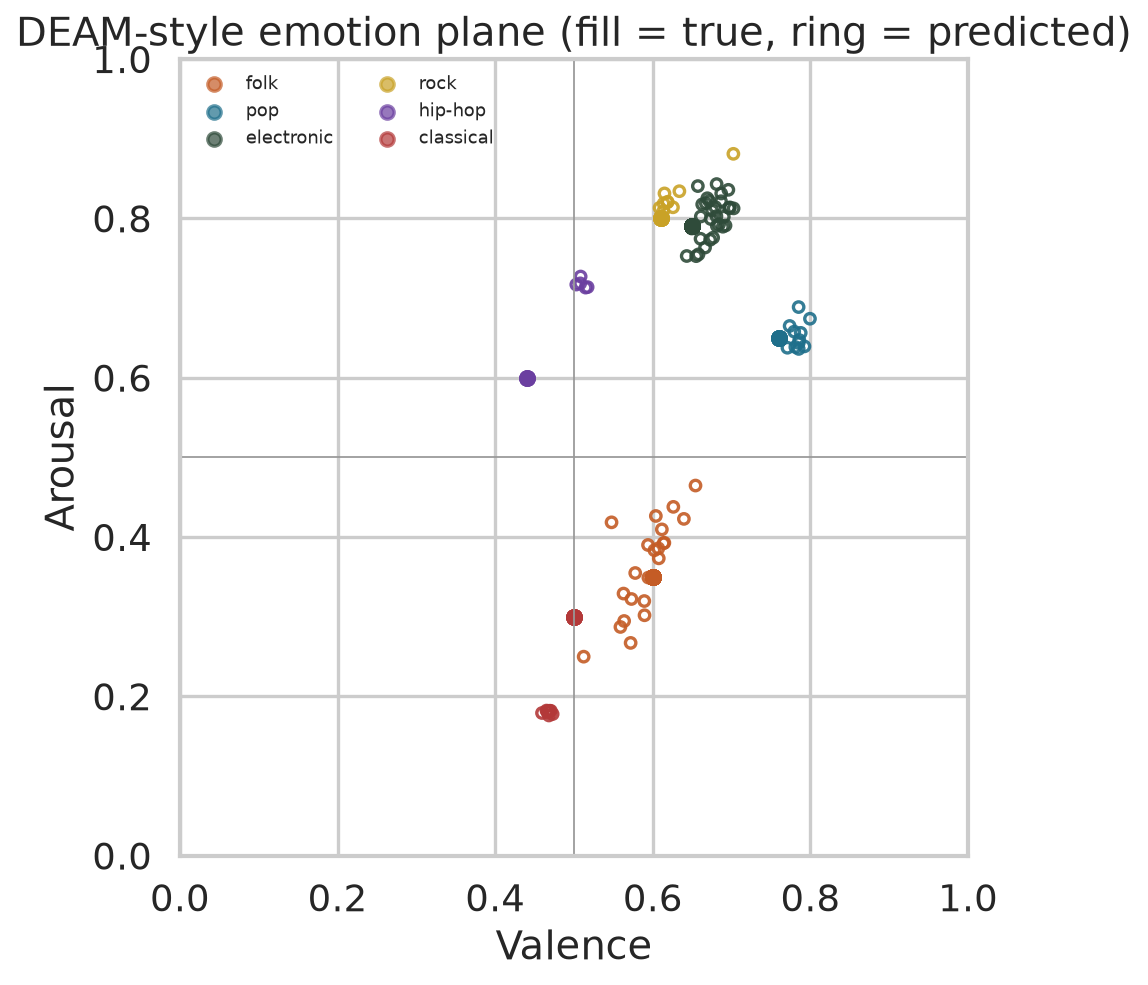
\includegraphics[width=\columnwidth,height=1.55in,keepaspectratio]{valence_arousal.png}
\caption{Valence--arousal plane (fill: true; ring: predicted). Targets are FMA-genre priors.}
\label{fig:va}
\end{figure}

\subsection{Qualitative Analysis}
Table~\ref{tab:qual} lists three held-out clips. Fusion copies metadata tags almost exactly, as expected given how labels are built, and recovers genre-prior VA. The GNN genre head is weaker: \emph{heartbreaker} (experimental/electronic) and \emph{110\%} (hip-hop) are both predicted as folk. Thirty-second chroma graphs at this capacity do not solve FMA-small genre. Graph coherence is the fraction of edges with feature cosine above $0.5$. Example tensors (12 clips $\times$ segment and chord $= 24$ files) load with \texttt{torch.load} and \texttt{weights\_only=False}.

\begin{table}[t]
\caption{Three test clips. Tags are metadata-derived; GNN genre is audio-only.}
\label{tab:qual}
\centering
\scriptsize
\renewcommand{\arraystretch}{1.2}
\setlength{\tabcolsep}{3pt}
\begin{tabularx}{\columnwidth}{@{}>{\raggedright\arraybackslash}p{1.5cm}>{\raggedright\arraybackslash}p{1.45cm}>{\raggedright\arraybackslash}X>{\raggedright\arraybackslash}p{2.05cm}@{}}
\toprule
Track & Caption & Tags true$\to$pred & Genre / VA \\
\midrule
000620 Arabesque & folk, Ed Askew & guitar, vocals, calm, acoustic $\to$ same & folk$\to$folk\newline $0.60/0.35\to0.57/0.27$ \\
007373 heartbreaker & electronic & drums, synth, bass, dark $\to$ drops dark & elec.$\to$folk\newline $0.65/0.79\to0.68/0.78$ \\
013749 110\% edit & hip-hop, Laws & drums, vocals, bass, minor\_key $\to$ same & hip-hop$\to$folk\newline $0.44/0.60\to0.50/0.72$ \\
\bottomrule
\end{tabularx}
\end{table}

\subsection{Error Analysis}
Two failure modes dominate. First, \emph{template leakage}: any model that sees the caption can recover tags that were extracted from that caption. That inflates BERT and fusion F1 relative to GNN and CNN. A fairer text task would use MusicCaps captions written independently of the tag inventory. Second, \emph{genre collapse} in the GNN: folk is the largest mapped class (128 clips) and international/folk chroma is a convenient attractor for short clips with acoustic spectra. Hip-hop and experimental electronics are the usual victims in Table~\ref{tab:qual}. Retrieval fails when two captions differ only in title tokens that TinyBERT may treat as rare UNKs after a 48-token cut.

\subsection{Limitations}
Fusion should help when a caption names an instrument the graph does not encode, and when the graph encodes a progression the caption only implies. On this subset the text tower dominates tags because labels are metadata-derived. Cross-attention does not beat concat until captions are longer and more compositional. Other limits: no DEAM ratings, no MagnaTagATune crowd tags, no jazz or metal top-genre buckets in FMA-small, 30\,s crops that under-represent long-range form, CPU-scale TinyBERT rather than a pretrained BERT checkpoint, and a 90-clip test split that makes R@1 a coin flip. We report the retrieval failure instead of hiding it.

\section{Implementation and Reproducibility}
The stack is Python~3.10, PyTorch, librosa, and NumPy. Official FMA dumps are SHA1-checked into a gitignored raw-audio directory. The same repository then builds the real corpus, trains all four tasks, writes metrics and plots, and compiles this PDF. No artist appears in two splits. Twelve saved graph identifiers are listed in the appendix.

\section{Conclusion}
We implemented the full four-task GNN--BERT music-context pipeline on official FMA-small audio, with majority, CNN, BERT, and GNN baselines, concat versus cross-attention, retrieval, and this report. Concat fusion is the best tagger on metadata-derived labels. Audio-only models show the real FMA difficulty. Retrieval stays near chance until captions become unique. Joining MusicCaps audio and DEAM ratings is the remaining upgrade for human text and emotion.

\appendix
\section{Graph Tensor Format}
Each saved sample is a Python dictionary written with \texttt{torch.save}: a $N\times 312$ node-feature matrix, a dense adjacency matrix, sparse edge indices and weights, string node labels (for example \texttt{seg0} or \texttt{Amin}), and a kind flag of segment or chord. Load with \texttt{weights\_only=False}. Segment graphs in this subset always have $N=30$; chord graphs vary with the estimated progression.

\section{Tag Mapping}
A tag fires if any synonym in Table~\ref{tab:syn} appears in the caption, FMA tag string, or leaf genre names. If fewer than three tags fire, the highest-prior tags from the mapped genre (piano/brass for jazz, guitar for folk, synth/drums for electronic, and so on) are filled until three positives exist. Genre-prior tags with probability $\ge 0.7$ are always on. This is why BERT F1 is high: the caption almost lists the tags.

\begin{table}[t]
\caption{Selected tag synonyms used by the keyword mapper.}
\label{tab:syn}
\centering
\scriptsize
\begin{tabular}{lp{5.6cm}}
\toprule
Tag & Fires on \\
\midrule
guitar & guitar, guitars, acoustic guitar, electric guitar \\
piano & piano, keys, keyboard \\
drums & drum, drums, beat, percussion \\
synth & synth, synthesizer, pad, analog \\
vocals & vocal, vocals, voice, singing, singer \\
melancholic & sad, melancholy, melancholic, wistful \\
energetic & energetic, energy, aggressive, intense \\
electronic\_prod & electronic, produced, studio \\
\bottomrule
\end{tabular}
\end{table}

The mapping is intentionally conservative. We do not run a separate audio tagging network to invent MagnaTagATune labels, because that would hide the fact that MTT audio is missing.

\section{Saved Graph Inventory}
Twelve clips export both graphs (24 files):
\texttt{fma\_000620}, \texttt{000690}, \texttt{000705}, \texttt{002099}, \texttt{003263}, \texttt{003271}, \texttt{003273}, \texttt{004066}, \texttt{004070}, \texttt{004108}, \texttt{004235}, \texttt{004519}.
A typical segment graph has 30 nodes and 50--80 undirected edges. A typical chord graph has 6--12 nodes. Remaining tag synonyms include strings (violin, cello, orchestra), bass (sub bass, 808), brass (horn, trumpet, sax), calm (quiet, soft, peaceful), dark (brooding, ominous), uplifting (happy, bright, cheerful), danceable (dance, club, groove), live (concert), 1960s (1960, 60s), modern (contemporary), fast\_tempo (uptempo), and slow\_tempo (ballad).

\section{Evaluation Formulae}
Let $y\in\{0,1\}^{N\times 24}$ be the test tags and $\hat p=\sigma(\ell)$ the sigmoid of the model logits. A tag is predicted positive if $\hat p_{ik}\ge 0.5$. Per-tag F1 is the harmonic mean of precision and recall; macro-F1 is the unweighted mean over 24 tags (zero-division is scored as 0). Micro-F1 pools true positives, false positives, and false negatives across tags before computing a single F1. AUC-PR is scikit-learn's \texttt{average\_precision\_score} on tags that occur at least once in the test split, then averaged (macro). Genre accuracy is $\frac1N\sum_i\mathbf{1}[\arg\max \ell_i^{\mathrm{gen}}=y_i^{\mathrm{gen}}]$. Emotion MAE is
\begin{equation}
\mathrm{MAE}_{\mathrm{emo}}=\tfrac12\big(\mathrm{MAE}_v+\mathrm{MAE}_a\big),
\end{equation}
with $R^2$ reported separately per axis. Retrieval Recall@$K$ is the fraction of queries whose paired item appears among the $K$ nearest $\ell_2$-normalized neighbours. Chance caption-to-audio R@$K$ on $N=90$ is $K/90$. Majority tags copy the train empirical frequency and threshold at $0.5$; random tags draw $U(0,1)$ scores (seed 0). These definitions match the evaluation and contrastive modules used for the tables.

\section{Feature Extraction}
Audio is loaded with librosa, resampled to $22\,050$\,Hz, converted to mono, and cropped to the first 30\,s of the file (or the full file if shorter). A missing or corrupt mp3 is skipped; one FMA-small file in the seed-42 subset failed this check. The STFT uses hop 512. Log-mel uses 128 bands; chroma is 12-bin; MFCCs are 13 coefficients. RMS, spectral centroid, and zero-crossing rate are stored as extra 1-d streams. Each clip is $z$-scored per feature tensor before graph construction.

A 30\,s crop at hop 512 yields about 1290 frames. Segment graphs slice those frames into non-overlapping 1\,s windows ($N=30$). Node $i$ concatenates mean and standard deviation of each stream over the window:
\begin{multline}
x_i=\big[\mu,\sigma\big]_{\mathrm{mel}}\,\|\,\big[\mu,\sigma\big]_{\mathrm{chroma}}\\
\|\,\big[\mu,\sigma\big]_{\mathrm{MFCC}}\,\|\,\big[\mu,\sigma\big]_{\mathrm{RMS,\,cent,\,ZCR}}.
\end{multline}
That is $2\times(128+12+13+3)=312$ dimensions (Table~\ref{tab:nodedim}). Similarity edges use only the chroma$\|$MFCC slice so timbre-only matches do not saturate the graph. The CNN baseline downsamples log-mel to $64\times 32$ before three convolutional blocks; it never sees the graph.

\begin{table}[t]
\caption{Segment-node feature layout ($312$ dimensions).}
\label{tab:nodedim}
\centering
\scriptsize
\begin{tabular}{lcc}
\toprule
Stream & Bands & Mean$+$std dims \\
\midrule
Log-mel & 128 & 256 \\
Chroma & 12 & 24 \\
MFCC & 13 & 26 \\
RMS / centroid / ZCR & 1+1+1 & 6 \\
Total & --- & 312 \\
\bottomrule
\end{tabular}
\end{table}

\section{Chord Templates}
Major and minor triads are 12-d templates with weights $(1.0,0.8,0.9)$ on root, third, and fifth (pitch classes $0,4,7$ for major and $0,3,7$ for minor). Rolling the template over 12 roots yields 24 rows, each $\ell_2$-normalized. Frame-wise chroma is $\ell_2$-normalized per column and scored by a matrix multiply; the argmax is the chord index in $\{0,\ldots,23\}$, named as \texttt{Cmaj} through \texttt{Bmin}. Consecutive identical indices collapse to one node; the node feature is the mean of the 312-d windows that carried that chord. Self-loops keep isolated chords in the graph. This is template matching, not a Viterbi decoder: we do not impose a key or a duration prior.

\section{Artist-Disjoint Splits}
Artists are sorted, shuffled with NumPy Generator seed $42+7$, and cut by the configured fractions $0.67/0.16/$rest. Every track of an artist follows that artist into exactly one of train, val, or test. The resulting clip counts on this FMA subset are 327 / 94 / 90. Because FMA-small has many one-track artists, the artist cut is close to a clip cut, but the invariant still holds: no test artist is seen in training. Ids are written with the artist-disjoint split. Evaluation never peeks at train logits when reporting Table~\ref{tab:results}.

\section{Training Protocol}
Each task is a separate AdamW run: 10 epochs for TinyBERT tags, 14 for GraphSAGE (genre and tags), CNN, and both fusion variants, and 16 for the dual encoder. BERT weights are copied into fusion when the Task~1 checkpoint exists. Graphs in a minibatch are padded to the longest $N$ with a boolean node mask. Checkpointing uses validation macro-F1, genre accuracy, R@5, or F1 minus an emotion-MAE penalty. Fig.~\ref{fig:f1} is the validation trace. All runs use seed 42 and CPU (PyTorch 2.14).

\section{Synthetic Fallback}
If FMA audio is not on disk, a 288-clip synthetic generator still builds a stand-in corpus (48 artists $\times$ 8 genres, 8\,s tones with genre-conditioned chord loops). Captions, tags, and VA are sampled from the same genre-prior table, so a synthetic run cannot diagnose template leakage against real FMA metadata. The numbers in this paper are from the 511-clip FMA subset, not from that generator. The generator remains so that unit tests run without a 7\,GB download.

\section{Licensing and Ethics}
\balance
FMA audio is Creative Commons; we do not redistribute the 7\,GB FMA-small zip or the decoded mp3s. Users re-fetch with the published SHA1. MusicCaps captions are released by Google; we store the public CSV and do not fetch YouTube audio. DEAM is gated, so we never claim human emotion labels. Captions that include artist and album names are metadata, not model-generated lyrics. No listener study was run. This is an engineering account of a 511-clip subset, not a production MIR system.

\section{Losses}
Task~1 and the GNN/CNN tag heads minimize binary cross-entropy on logits,
\begin{equation}
\mathcal{L}_{\mathrm{tag}}=-\frac1{24N}\sum_{i,k}\big[y_{ik}\log\sigma(\ell_{ik})+(1-y_{ik})\log(1-\sigma(\ell_{ik}))\big].
\end{equation}
The GNN and CNN genre heads use softmax cross-entropy over eight classes. Fusion adds the emotion term $\alpha\|v-\hat v\|_2^2+\beta\|a-\hat a\|_2^2$ with $\alpha=\beta=0.35$; valence and arousal heads are linear. Contrastive training uses the symmetric InfoNCE in~(6). No scheduled learning-rate decay is applied; AdamW's default $\beta$ and $\epsilon$ are kept. Gradient clipping is not used. Dropout $0.15$ is the only regularizer besides weight decay.

\section{Saved Artifacts}
Table~\ref{tab:art} lists the files a fresh clone must produce to reproduce the numbers in this paper. Raw audio is never committed. Unit tests cover chord templates, GraphSAGE shapes, InfoNCE numerics, FMA caption helpers, and loading a saved graph. They do not retrain models.

\begin{table}[t]
\caption{Artifacts written by the FMA run (audio excluded).}
\label{tab:art}
\centering
\scriptsize
\renewcommand{\arraystretch}{1.15}
\begin{tabularx}{\columnwidth}{@{}>{\raggedright\arraybackslash}X>{\raggedright\arraybackslash}X@{}}
\toprule
Path & Produced by \\
\midrule
\texttt{corpus.npz}, \texttt{vocab.json} & corpus / Task~1 \\
\texttt{splits.json} & artist-disjoint split \\
\texttt{graphs/fma\_*} & 24 example graphs \\
\texttt{checkpoints/*.pt} & training \\
\texttt{metrics.json}, plots & evaluation \\
\texttt{final\_report.pdf} & this paper \\
\bottomrule
\end{tabularx}
\end{table}

\section{What Would Change With Held-Out Labels}
Two substitutions would change the interpretation of Table~\ref{tab:results} without touching the model code. First, replacing metadata captions with MusicCaps-style independent descriptions would stop tags from being a near-copy of the text; BERT F1 should fall toward the audio-only band unless the encoder actually grounds instruments in the spectrogram. Second, replacing genre-prior VA with DEAM human ratings would raise emotion MAE: a 30\,s FMA crop is not annotated for mood, and the current $R^2$ largely measures recovery of Table~\ref{tab:genre}'s prior. Retrieval would also benefit from unique captions; stereotyped FMA templates make InfoNCE a near-random ranking of 90 similar strings. Those datasets are not on disk in this environment, so we report the FMA run as-is rather than simulating them.

The assignment also names jazz and metal. They remain valid heads in the 8-way classifier, but FMA-small's eight top genres do not include them, so the corresponding rows of the confusion matrix are empty. Collecting FMA-medium jazz/metal or GTZAN would populate those heads.

\begin{thebibliography}{8}
\bibitem{devlin2019} J.~Devlin, M.~Chang, K.~Lee, and K.~Toutanova, ``BERT: Pre-training of deep bidirectional transformers for language understanding,'' in \emph{Proc.\ NAACL}, 2019.
\bibitem{hamilton2017} W.~Hamilton, Z.~Ying, and J.~Leskovec, ``Inductive representation learning on large graphs,'' in \emph{Proc.\ NeurIPS}, 2017.
\bibitem{velickovic2018} P.~Veli{\v{c}}kovi{\'c} \emph{et al.}, ``Graph attention networks,'' in \emph{Proc.\ ICLR}, 2018.
\bibitem{oord2018} A.~van den Oord, Y.~Li, and O.~Vinyals, ``Representation learning with contrastive predictive coding,'' arXiv preprint 1807.03748, 2018.
\bibitem{defferrard2017} M.~Defferrard, K.~Benzi, P.~Vandergheynst, and X.~Bresson, ``FMA: A dataset for music analysis,'' in \emph{Proc.\ ISMIR}, 2017.
\bibitem{law2009} E.~Law, K.~West, M.~Mandel, M.~Bay, and J.~S.~Downie, ``Evaluation of algorithms using games: The case of music tagging,'' in \emph{Proc.\ ISMIR}, 2009.
\bibitem{agostinelli2023} A.~Agostinelli \emph{et al.}, ``MusicLM: Generating music from text,'' arXiv preprint 2301.11325, 2023.
\bibitem{aljanaki2017} A.~Aljanaki, Y.-H.~Yang, and M.~Soleymani, ``Developing a benchmark for emotional analysis of music,'' \emph{PLOS ONE}, 2017.
\end{thebibliography}

\end{document}
